\section{Analog-Digital-Wandler (ADC)}
\todo{Woche 5, 19.10.21 und Repitition Woche 6}
\subsection{Flash-Wandler (Parallelverfahren)}
Schnell und einfach, aber braucht sehr viel Platz.

\subsection{Pipeline-Wandler}
haben gleichen Datendurchsatz wie Flash-Wandler, haben aber Latenz da mehrstufig

\subsection{Successsive Approximation Register (SAR, Wägeverfahren)}
\includegraphics[width=\columnwidth]{Images/wägeverfahren_adc}

\subsection{Integrierende Verfahren (Dual Slope, Zählverfahren)}
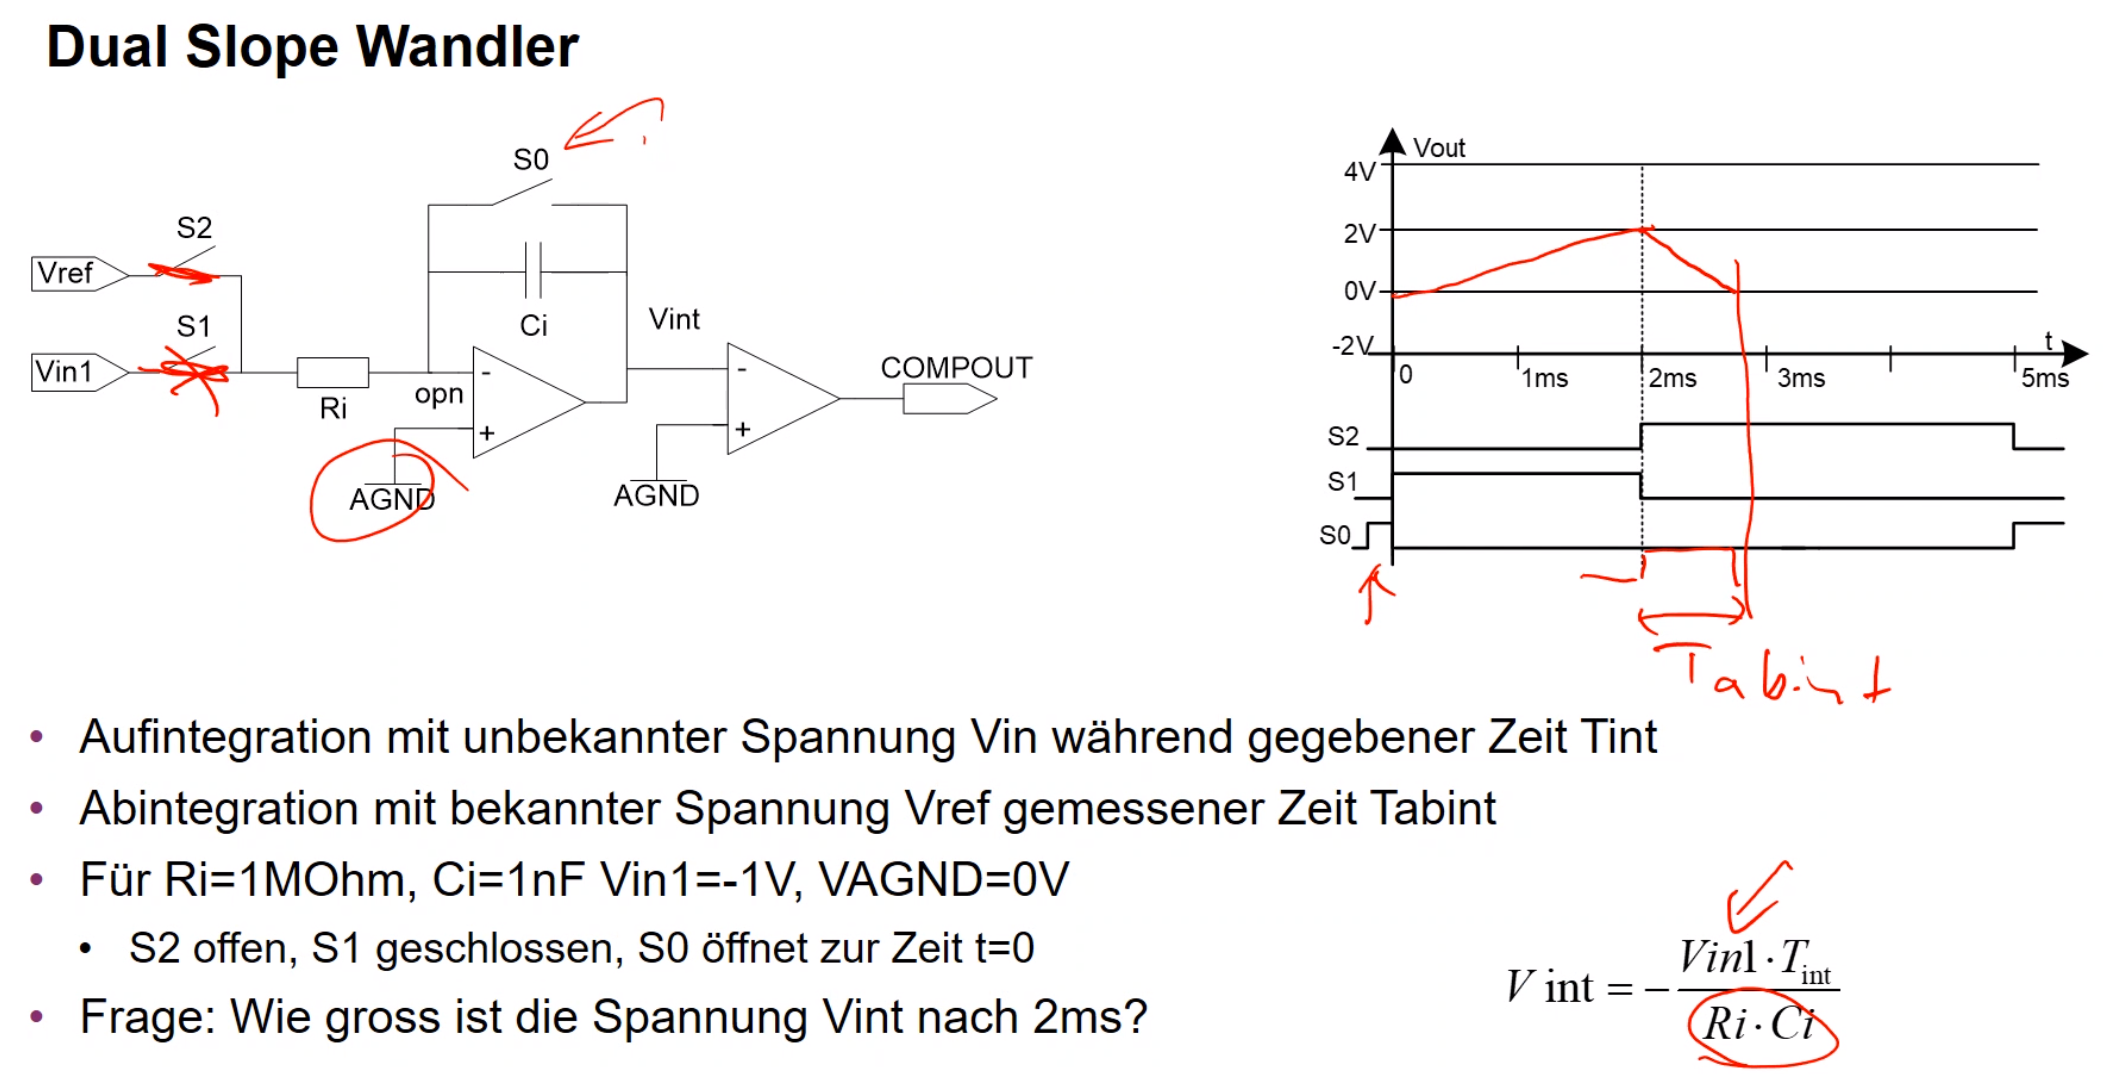
\includegraphics[width=\columnwidth]{Images/dual_slop_adc}
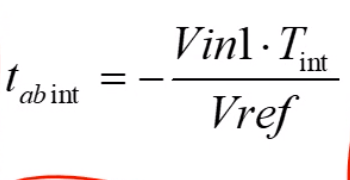
\includegraphics[width=0.2\columnwidth]{Images/dual_slop_adc1_2}


\subsection{Fehler}

\begin{enumerate}[nosep]
	\item Gleich wie DAC
	\item Aperturfehler
	\item Alaising
\end{enumerate}